\documentclass[x11names]{report}
\usepackage[a4paper, total={6in, 9in}]{geometry}
\usepackage[skins]{tcolorbox}
\usepackage{tikz}
\usetikzlibrary{arrows}
\usetikzlibrary{calc}
\usepackage{pgfplots}
\pgfplotsset{compat=1.9}
\usepgflibrary{shapes.geometric}
\usepackage{xcolor}
\usepackage{amsmath}
%\usepackage{fouriernc}
\usepackage{mathrsfs}
\usepackage{amssymb}
\usepackage{hyperref}

%% custom
\renewcommand*\contentsname{Indice}
\setcounter{tocdepth}{4}
\setcounter{secnumdepth}{2}
\pgfplotsset{compat=1.15}

\usepackage[pagestyles]{titlesec}
\titleformat{\chapter}[display]{\normalfont\bfseries}{}{0pt}{\Huge}
\newpagestyle{mystyle}
{\sethead[\thepage][][\chaptertitle]{}{}{\thepage}}
\pagestyle{mystyle}


% boxes
\definecolor{myblue}{RGB}{224, 245, 255} 
\definecolor{myred}{RGB}{198, 247, 211} 
\definecolor{myorange}{RGB}{255, 102, 0} 
\definecolor{mypurple}{RGB}{255, 102, 0} 

\newtcolorbox{es}[2][]{%
	enhanced,sharp corners,boxrule=0.4pt,colback=white, colframe=black, coltitle=black,fonttitle=\itshape, 
	attach boxed title to top left={yshift=-0.5\baselineskip-0.4pt,xshift=2mm},
	boxed title style={tile, size=minimal, left=0.5mm, right=0.5mm,
		colback=white, before upper=\strut, boxrule=0.5pt, colframe=black},
	title=#2,top=1em,#1 
}
\newtcolorbox{dym}[2][]{%
	enhanced,colback=white,colframe=black,coltitle=black,
	sharp corners,boxrule=0pt, %0.4pt
	fonttitle=\itshape,,
	attach boxed title to top left={yshift=-0.5\baselineskip-0.4pt,xshift=2mm},
	boxed title style={tile,size=minimal,left=2.5mm,right=0.5mm,
		colback=white,before upper=\strut},
	title=#2,top=1em,#1
}
\newtcolorbox{blues}[2][]{%
	enhanced,colback=myblue,colframe=black,coltitle=black,
	sharp corners,boxrule=0.4pt,
	fonttitle=\bfseries\itshape,
	attach boxed title to top left={yshift=-0.5\baselineskip-0.4pt,xshift=2mm},
	boxed title style={tile,size=minimal,left=0.5mm,right=0.5mm,
		colback=myblue,before upper=\strut},
	title=#2,top=1em,#1
}
\newtcolorbox{redes}[2][]{%
	enhanced,colback=myred,colframe=black,coltitle=black,
	sharp corners,boxrule=0.4pt,
	fonttitle=\bfseries\itshape,
	attach boxed title to top left={yshift=-0.5\baselineskip-0.4pt,xshift=2mm},
	boxed title style={tile,size=minimal,left=0.5mm,right=0.5mm,
		colback=myred,before upper=\strut},
	title=#2,top=1em,#1
}
\newtcolorbox{coroll}[2][]{%
	enhanced, colback=white, colframe=black, coltitle=black,
	sharp corners, boxrule=0pt,
	fonttitle=\bfseries\itshape,
	attach boxed title to top left={yshift=-0.5\baselineskip-0.4pt,xshift=2mm},
	boxed title style={tile,size=minimal,
		left=1mm, right=1mm, % Horizontal padding
		top=1mm, bottom=1mm, % Vertical padding
		colback=myred,
		before upper=\strut},
	title=#2,top=1em,#1
}

\newcommand*{\QEDA}{\null\nobreak\hfill\ensuremath{\blacksquare}}%
\newcommand*{\QEDB}{\null\nobreak\hfill\ensuremath{\square}}%

\newcommand{\esempio}[2]{
	\begin{es}{esempio #1}
		#2
	\end{es}
}
\newcommand{\definizione}[2]{
	\begin{center}
		\fboxsep11pt
		\colorbox{myblue}{\begin{minipage}{5.75in}
				\begin{blues}{Definizione: #1}
					#2
				\end{blues}
		\end{minipage}}
	\end{center}
}
\newcommand{\teorema}[2]{
	\begin{center}
		\fboxsep11pt
		\colorbox{myred}{\begin{minipage}{5.75in}
				\begin{redes}{#1}
					#2
				\end{redes}
		\end{minipage}}
	\end{center}
}
\newcommand{\dimostrazione}[2]{
	\begin{dym}{dimostrazione#1}
		#2
		\QEDB
	\end{dym}
}
\newcommand{\corollario}[2]{
	\begin{center}
		\begin{coroll}{corollario#1}
			#2
		\end{coroll}
	\end{center}
}

\newcommand{\verde}[1]{\colorbox{myred}{$\displaystyle #1$}}

\pgfplotsset{my axis/.append style={height=9cm,width=9cm,grid=major,samples=100,yticklabel=\empty,xticklabel=\empty}}
\pgfplotsset{my plot/.append style={thick,samples=500}}

\begin{document}
	
\begin{titlepage}
	\begin{center}
		\vspace*{1cm}
		
		\textbf{\LARGE Relazione di laboratorio - Pendolo semplice}
		
		\vspace{0.3cm}
		\large \textit{Misura del periodo di un pendolo semplice} \\
		
		\vspace{0.5cm}
		\Large Federico Cesari \\
		
		\small 1096759 
		\vspace{0.2cm}
		
		\small Gruppo 5
		
		
		\vspace{3cm}
		\begin{center}
			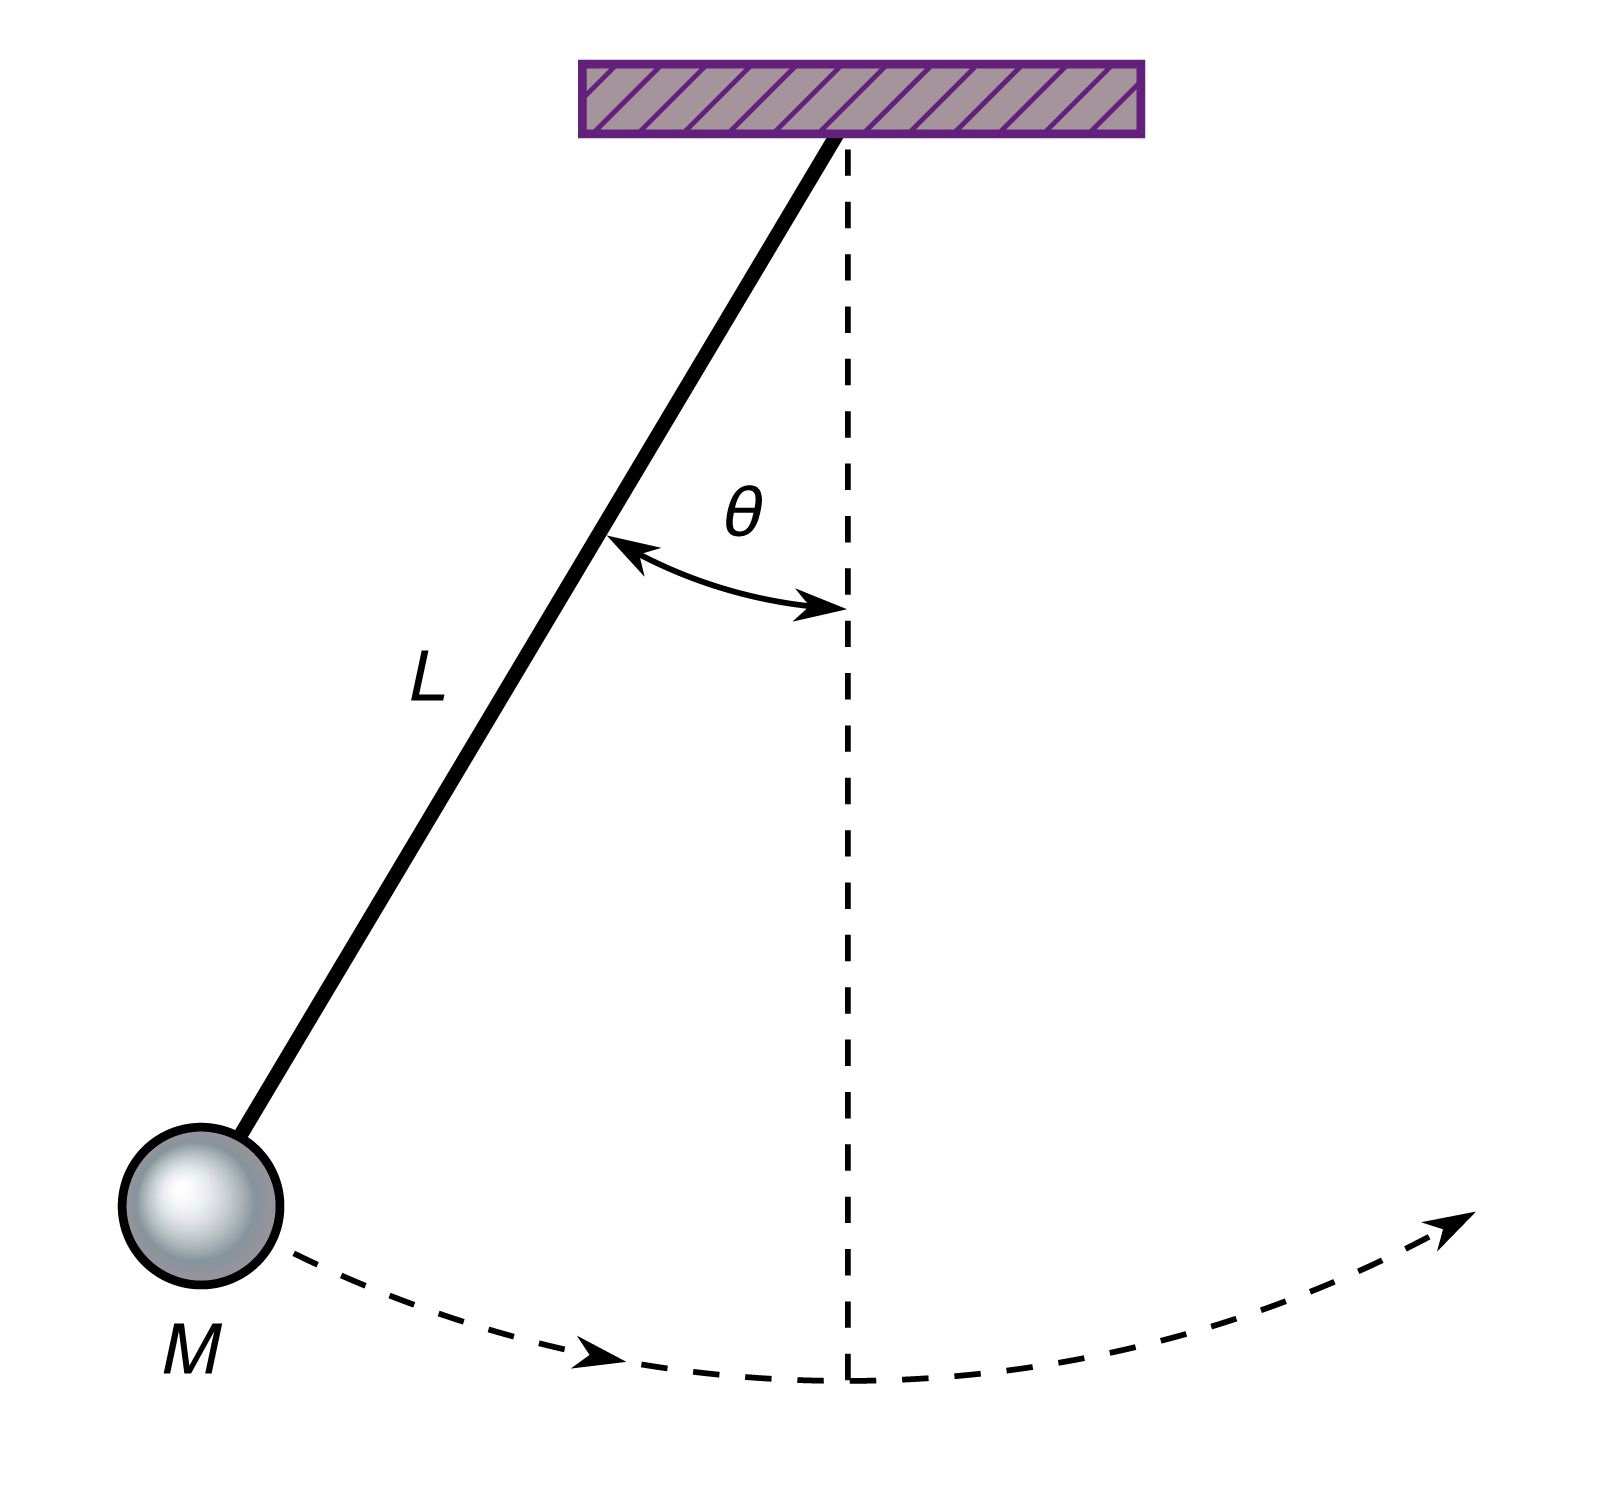
\includegraphics[scale=0.1]{IMG_0200.jpeg}	
		\end{center}
		
		
		
		\vfill
		
		
		
		corso A\\
		Università degli studi di Torino, Torino\\
		4 aprile 2024\\
		
		
	\end{center}
\end{titlepage}
\tableofcontents
\newpage
	
\chapter{Elettrostatica}
\section{Campo elettrico}
\subsection{Dipolo elettrico}
Definiamo \textbf{momento del dipolo}
\[
\vec{p} = q\vec{a}
\]
Consideriamo un punto \(P\) nel quale misuriamo il potenziale, pari alla somma dei contributi delle due cariche:
\[
V(P) = \frac{q}{4\pi \varepsilon_0} \left(\frac{1}{r_1} - \frac{1}{r_2}\right) = \frac{q}{4\pi \varepsilon_0} \left(\frac{r_2 - r_1}{r_1r_2}\right)
\]
Ipotizziamo che \(P\) sia molto distante dal dipolo (rispetto alla distanza \(a\)) così che \(r_1\) e \(r_2\) siano sempre più assimilabili a due segmenti paralleli. Andiamo poi a tracciare un segmento perpendicolare a \(r_1\) fino a \(r_2\) evidenziando la distanza \(r_2 - r_1 \approx a\cos\vartheta\). 

\subsubsection{Potenziale del dipolo}
Con le seguenti approssimazioni andiamo a riscrivere il potenziale:
\[
r_2 - r_1 \approx a\cos\vartheta \qquad \qquad r_1r_2 \approx r^2
\]
\[
V(P) = \frac{q}{4\pi \varepsilon_0} \left(\frac{a\cos\vartheta}{r^2}\right) = \frac{p}{4\pi \varepsilon_0 r^2}
\]
Vediamo come a grandi distanze il potenziale del punto \(P\) dia \textit{informazioni solo sul momento di dipolo} e non sulle due cariche o sulla loro distanza reciproca. A parità di momento si potranno avere due cariche ravvicinate e molto cariche o più distanti e meno cariche.


\subsubsection{Campo elettrico del dipolo}
Riscrivendo \(r\) e \(\cos\vartheta\) esprimiamo il potenziale come
\[
V(P) = \frac{q}{4\pi \varepsilon_0} \left(\frac{a\textcolor{orange}{\cos\vartheta}}{\textcolor{red}{r^2}}\right) 
\]
\[
V(P)= \frac{p}{4\pi\varepsilon_0}\frac{1}{\textcolor{red}{x^2 + y^2 + z^2}}\textcolor{orange}{\frac{z}{\sqrt{x^2 + y^2 + z^2}}} = \frac{p}{4\pi\varepsilon_0}\frac{z}{(x^2+y^2+z^2)^{\frac{3}{2}}}
\]\\

\noindent
Dalla relazione \(\vec{E} = -\vec{\nabla}V\) otteniamo l'espressioni del campo elettrico
\[
\vec{E} = \left( \frac{p}{4\pi\varepsilon_0}\frac{3xz}{r^5},\;\ \frac{p}{4\pi\varepsilon_0}\frac{3yz}{r^5},\;\ \frac{p}{4\pi\varepsilon_0}\left(\frac{3z^2}{r^5}-\frac{1}{r^3}\right)\right) 
\]

\[
E(P) = \frac{p}{4\pi\varepsilon_0r^3}\sqrt{3\cos^2\vartheta + 1}
\]
Concludiamo osservando che il campo elettrico del dipolo varia con \(r^3\) (il monopolo con \(r^2\)) e dipende anche dall'angolo \(\vartheta\).



\section{Flusso di campo elettrico}
Definiamo flusso di un campo vettoriale \(\vec{E}\) l'integrale
\[
\Phi (\vec{E}) = \int_{\Sigma} \vec{E}\cdot \hat{u}_n \: d\Sigma
\]
dove \(\hat{u}_n\) è il versore normale alla porzione infinitesima di superficie \(d\Sigma\). Vediamo che il prodotto scalare fa sì che contribuisca solo la componente di campo vettoriale ortogonale alla superficie. 

Mostriamo come il flusso \textit{dipenda solo dall'angolo solido sotto il quale la superficie vede la carica}. Prima di tutto qualche osservazione geometrica:

\[
d\vartheta = \frac{ds}{r} \qquad \qquad ds' \cos\alpha = ds \;\ \to \;\ d\vartheta = \frac{ds'\cos\alpha}{r}
\]
\[
d\Omega= \frac{d\Sigma_0}{r^2} \qquad \qquad d\Sigma \cos\alpha = d\Sigma_0 \;\ \to \;\ d\Omega = \frac{d\Sigma\cos\alpha}{r^2}
\]
Andiamo ora a calcolare il flusso attraverso \(d\Sigma\):
\begin{align*}
	d\Phi =& \vec{E} \cdot \hat{u}_n d\Sigma \\ 
		  =& \frac{q}{4\pi\varepsilon_0 r^2} \hat{u}_r \cdot \hat{u}_n \: d\Sigma \\
		  =& \frac{q}{4\pi\varepsilon_0 r^2} |\hat{u}_r||\hat{u}_n|\textcolor{red}{\cos\alpha\: d\Sigma} \\ 
		  =& \frac{q}{4\pi\varepsilon_0 r^2} |\hat{u}_r||\hat{u}_n|\textcolor{red}{\: d\Sigma_0} \\
		  =& \frac{q}{4\pi\varepsilon_0  \textcolor{orange}{r^2}} \textcolor{orange}{\: d\Sigma_0} \\
		  =& \frac{q}{4\pi\varepsilon_0}\: \textcolor{orange}{d\Omega} \quad \to \quad \Phi = \frac{q}{4\pi\varepsilon_0}\Omega
\end{align*}
Quindi se consideriamo una superficie chiusa si ha un angolo solido
\[
d\Omega = \frac{4\pi r^2}{r^2} = 4\pi
\]
e di conseguenza
\begin{equation}
	\verde{\Phi = \frac{q}{\varepsilon_0}}
\end{equation}
Se la carica esterna il flusso è nullo (le cariche esterne contribuiscono solo al campo elettrico). Inoltre se consideriamo più cariche, o addirittura una distribuzione omogenea di cariche si hanno i seguenti valori di flusso:
\[
\text{distribuzione finita di cariche: }\qquad \Phi = \oint \vec{E} \cdot \hat{u}_n \: d\Sigma \;\ = \;\ \sum_i \frac{q_{i(int)}}{\varepsilon_0}
\]
\[
\text{distribuzione continua di cariche: }\qquad \Phi = \frac{1}{\varepsilon_0}\int \rho(x,y,z) \:d\tau 
\]




\subsubsection*{Rotore di un campo vettoriale}
Viene definito rotore del campo elettrico \(\vec{E}\) il prodotto vettoriale
\[
\vec{\nabla} \wedge \vec{E} = \left|\begin{array}{ccc}
	\hat{u}_x & \hat{u}_y & \hat{u}_z \\
	\frac{\partial}{\partial x} & \frac{\partial}{\partial y} & \frac{\partial}{\partial z} \\
	E_x & E_y & E_z 
\end{array}\right| = \left(\frac{\partial E_z}{\partial y}-\frac{\partial E_y}{\partial z}\right)\hat{u}_x + \left(\frac{\partial E_x}{\partial z}-\frac{\partial E_z}{\partial x}\right)\hat{u}_y + \left(\frac{\partial E_y}{\partial x}-\frac{\partial E_x}{\partial y}\right)\hat{u}_z
\]
Questo rappresenta la capacità del campo elettrico di \textit{formare vortici}, ovvero di generare linee di forza che si richiudono su loro stesse.


Poiché anche il rotore del campo elettrico è un campo vettoriale, è possibile definirne un suo flusso:

\[
\Phi(\vec{\nabla} \wedge \vec{E}) =  \int_{\Sigma}\left(\vec{\nabla} \wedge \vec{E}\right)\cdot \hat{u}_n \: d\Sigma
\]

\teorema{}{
\subsubsection{Teorema di Stokes}
La circuitazione è uguale al flusso del rotore:
\[
\oint_\gamma \vec{E}\cdot d\vec{s} = \int_{\Sigma_\gamma}\left(\vec{\nabla} \wedge \vec{E}\right)\cdot \hat{u}_n \: d\Sigma
\]
Qui è espresso nel caso del campo elettrico dove si ha che la circuitazione è nulla qualunque sia la curva \(\gamma\) (a patto che sia chiusa). Allora il flusso del rotore è nullo qualunque sia la superficie ed è possibile solo se il rotore di \(\vec{E}\) è nullo:

\[
\vec{\nabla} \wedge \vec{E} = 0
\]

Dire che il rotore è nullo equivale a dire che il capo elettrico è \textbf{irrotazionale}, ovvero che le sue linee di forza non possono chiudersi su loro stesse; il campo elettrico "non forma vortici".
}

L'annullarsi del rotore non è un fatto sorprendente. Sappiamo infatti che il rotore di un gradiente è sempre nullo e che il campo elettrostatico conservativo può essere scritto come gradiente della funzione scalare del potenziale elettrostatico \(V\):
\[
\vec{\nabla} \wedge \vec{E} = \vec{\nabla} \wedge \left(-\vec{\nabla} V\right)
\]

\subsection{Discontinuità di carica}


\end{document}